\section{常微分方程数值解}

见 Fiddie 讲义 11,12,13

\subsection{单步法}

\begin{figure}[H]
\centering
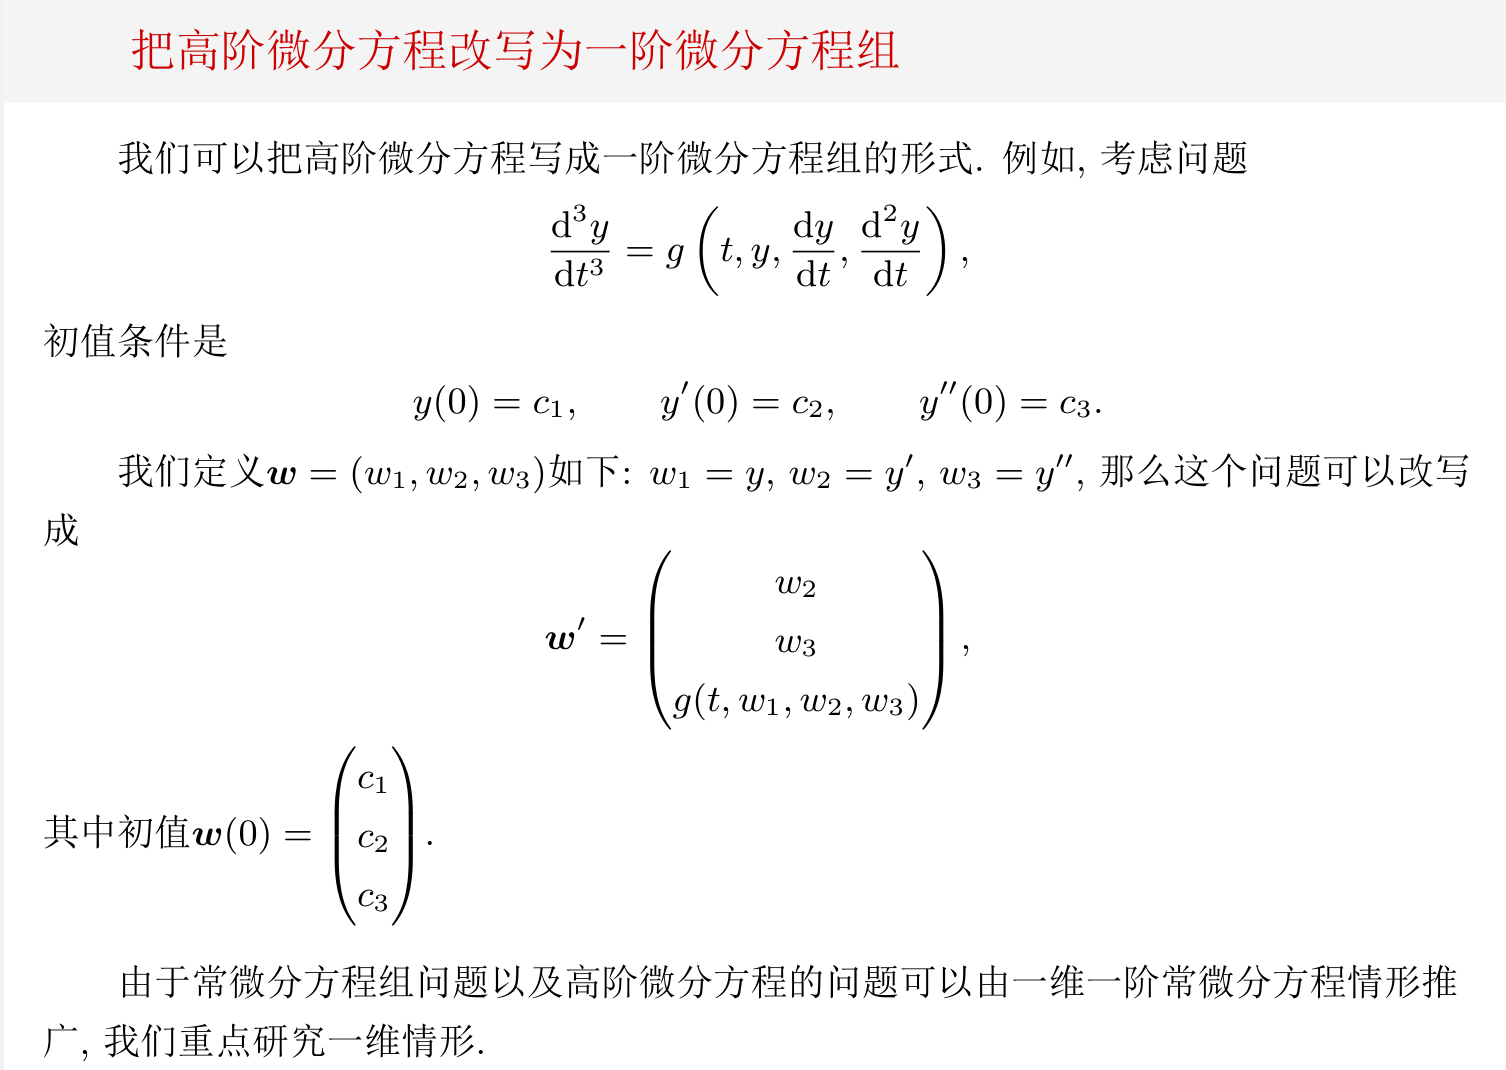
\includegraphics[width=\textwidth]{常微分方程数值解-2025051512.png}
% \caption{}
\label{}
\end{figure}

\begin{figure}[H]
\centering
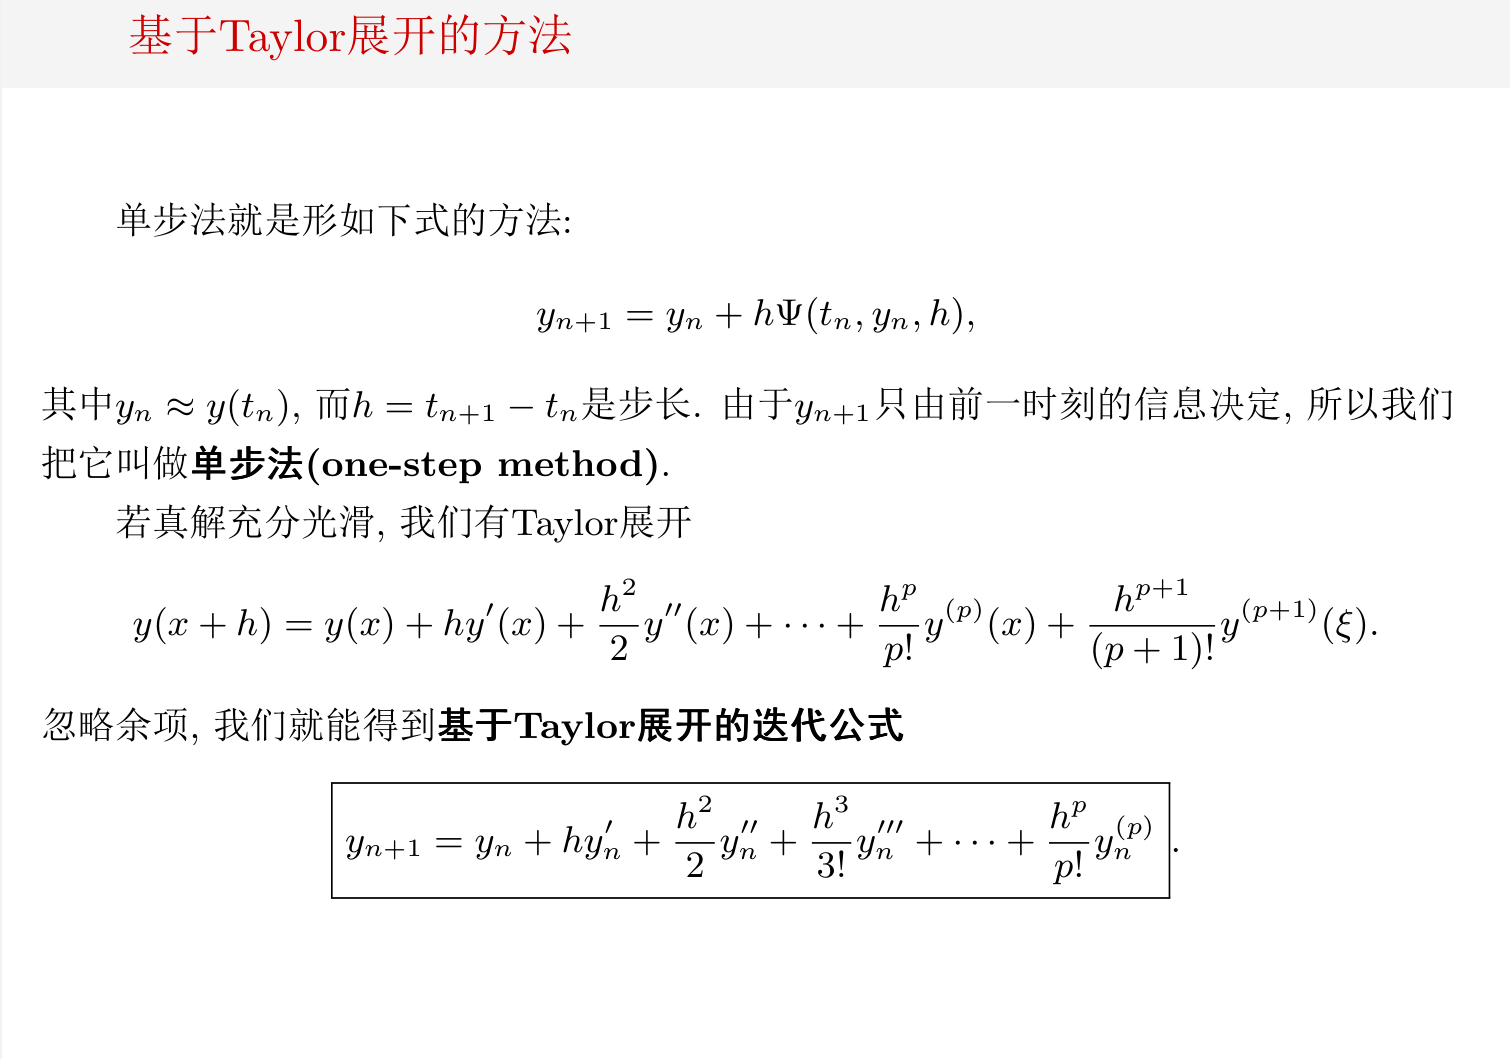
\includegraphics[width=\textwidth]{1-常微分方程数值解-2025051512.png}
% \caption{}
\label{}
\end{figure}
\begin{figure}[H]
\centering
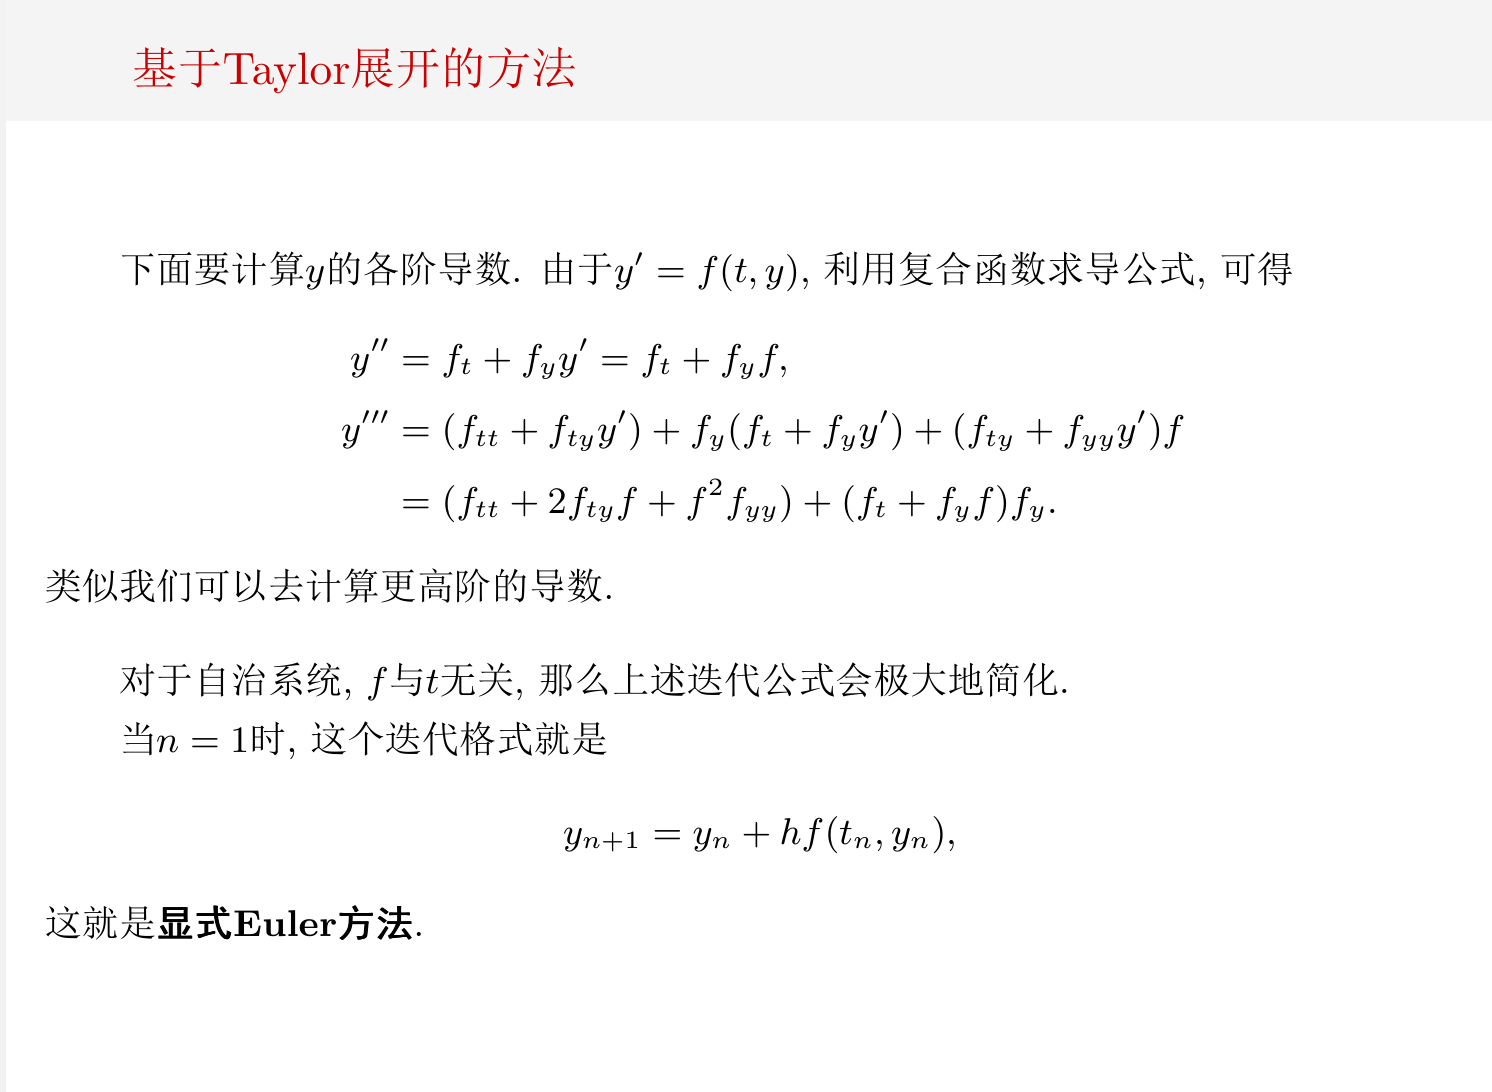
\includegraphics[width=\textwidth]{2-常微分方程数值解-2025051512.png}
% \caption{}
\label{}
\end{figure}

自治系统就是
\[
\boldsymbol{y}'=\boldsymbol{f}(t,\boldsymbol{y})
\]
其中 $\boldsymbol{f}(t,\boldsymbol{y})=f(\boldsymbol{y})$ 与 $t$ 无关.

\begin{figure}[H]
\centering
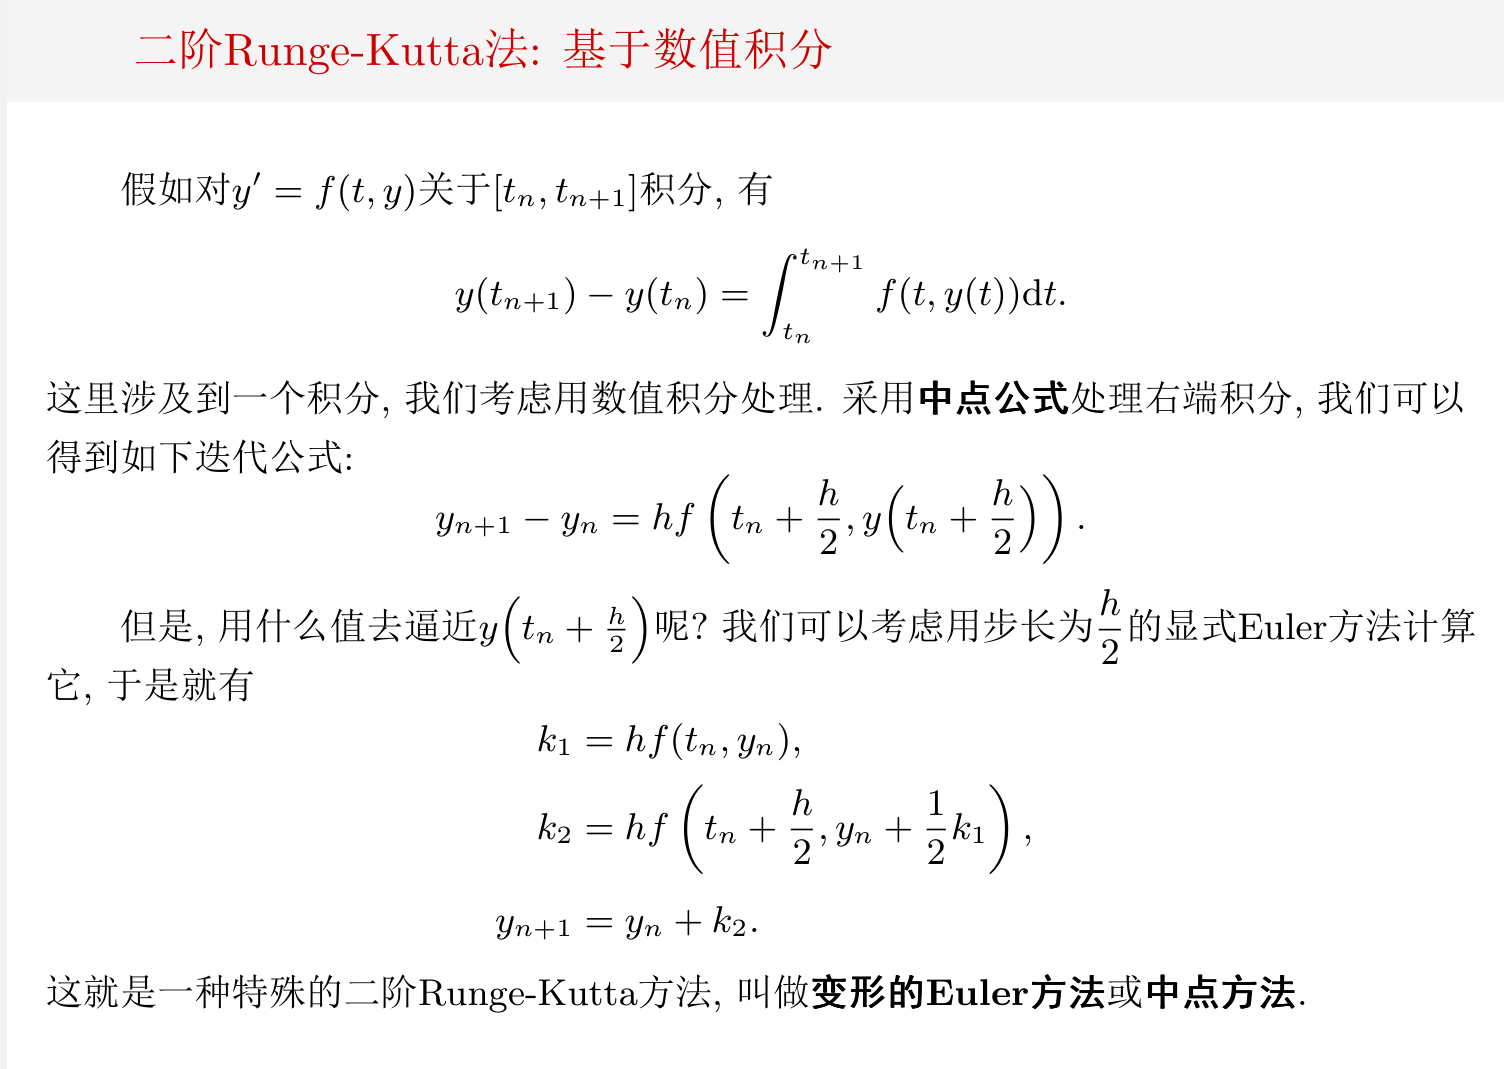
\includegraphics[width=\textwidth]{3-常微分方程数值解-2025051512.png}
% \caption{}
\label{}
\end{figure}

\begin{figure}[H]
\centering
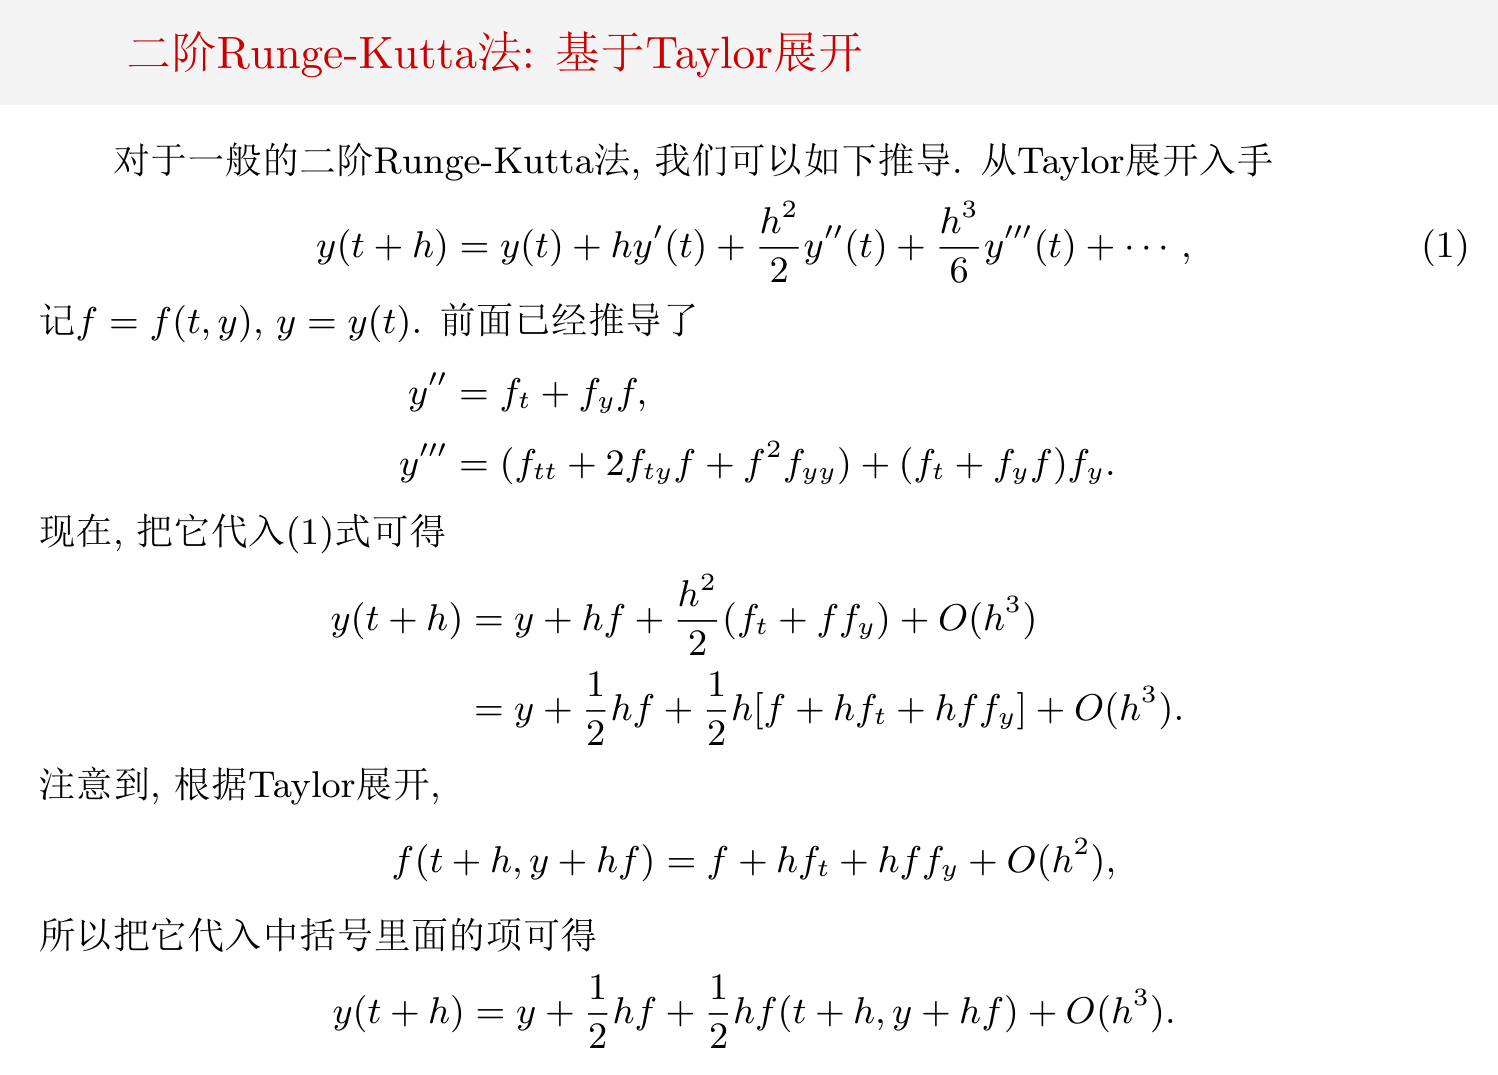
\includegraphics[width=\textwidth]{5-常微分方程数值解-2025051512.png}
% \caption{}
\label{}
\end{figure}

\begin{figure}[H]
\centering
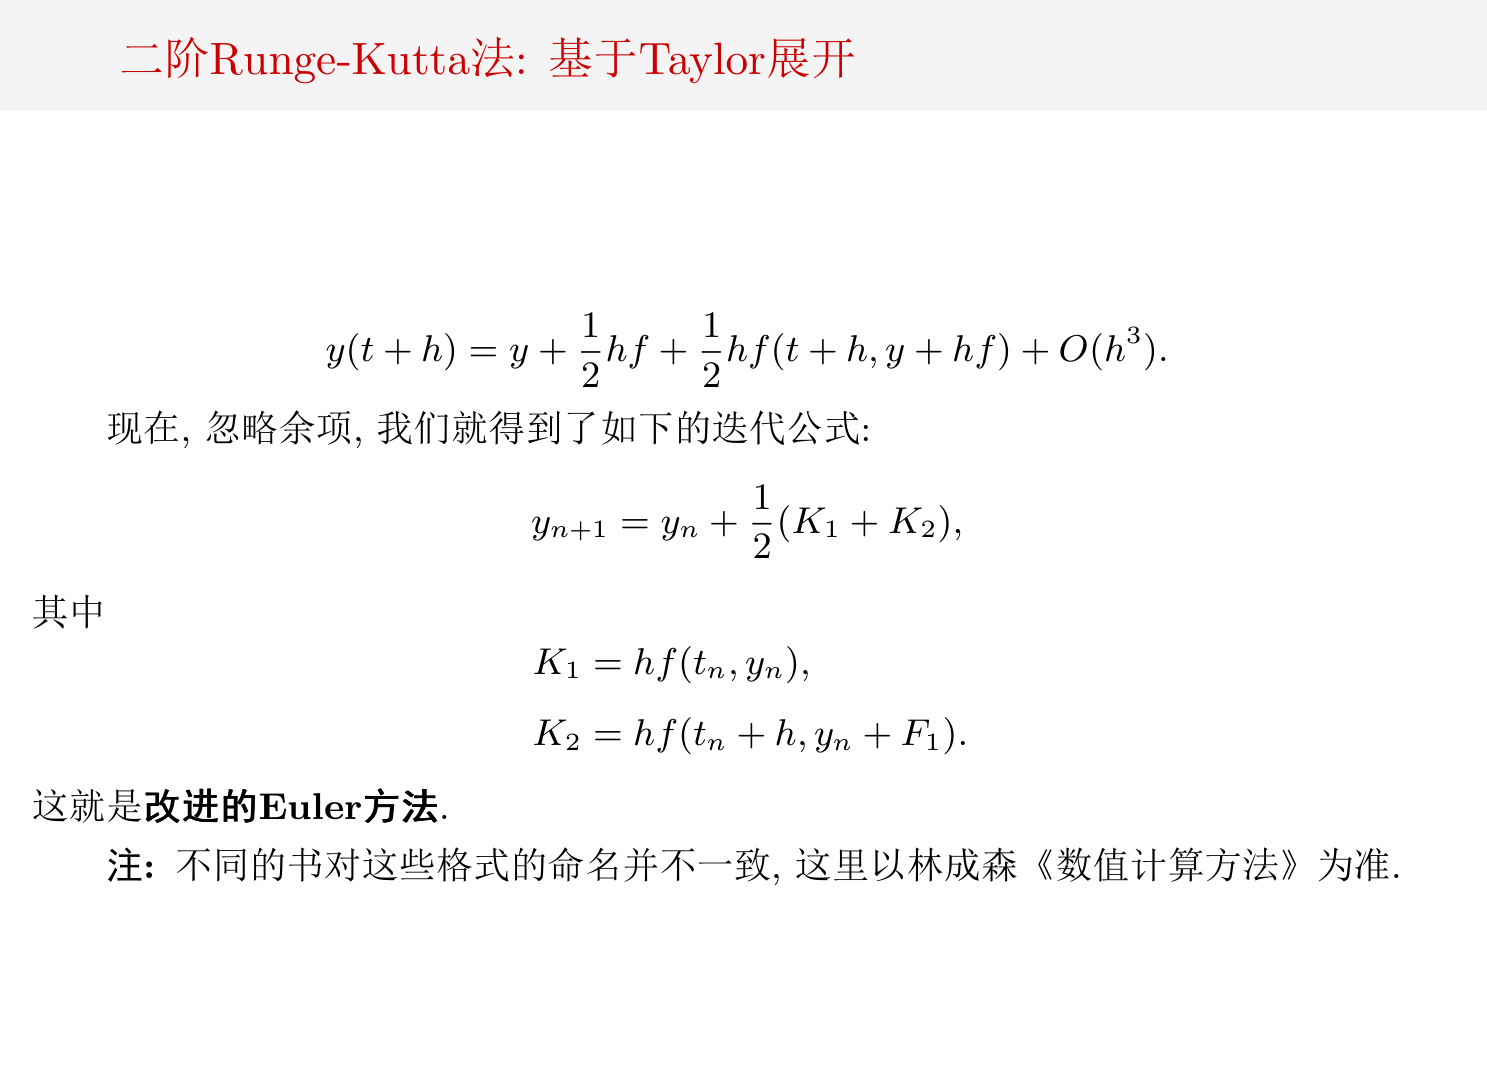
\includegraphics[width=\textwidth]{6-常微分方程数值解-2025051512.png}
% \caption{}
\label{}
\end{figure}

\subsection{单步法的相容性、收敛性、稳定性}

\begin{figure}[H]
\centering
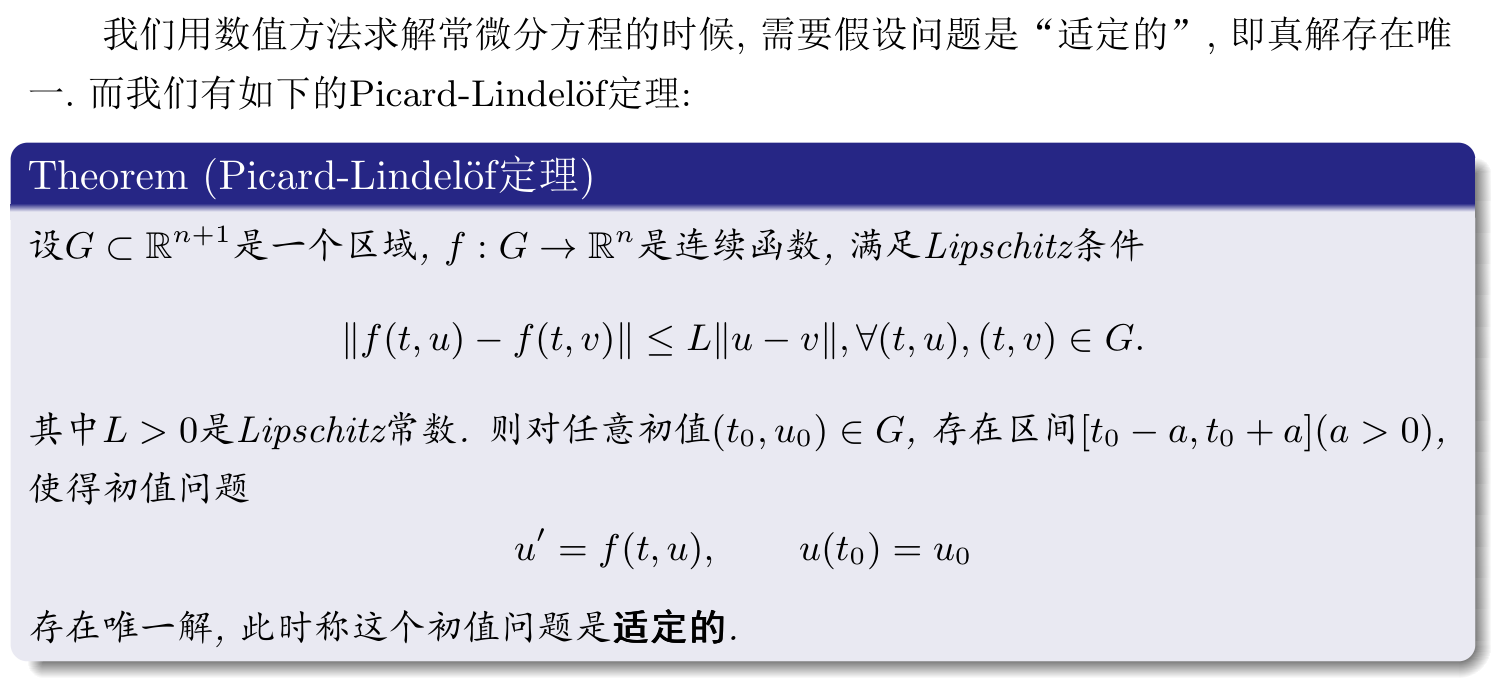
\includegraphics[width=\textwidth]{7-常微分方程数值解-2025051512.png}
% \caption{}
\label{}
\end{figure}

\begin{figure}[H]
\centering
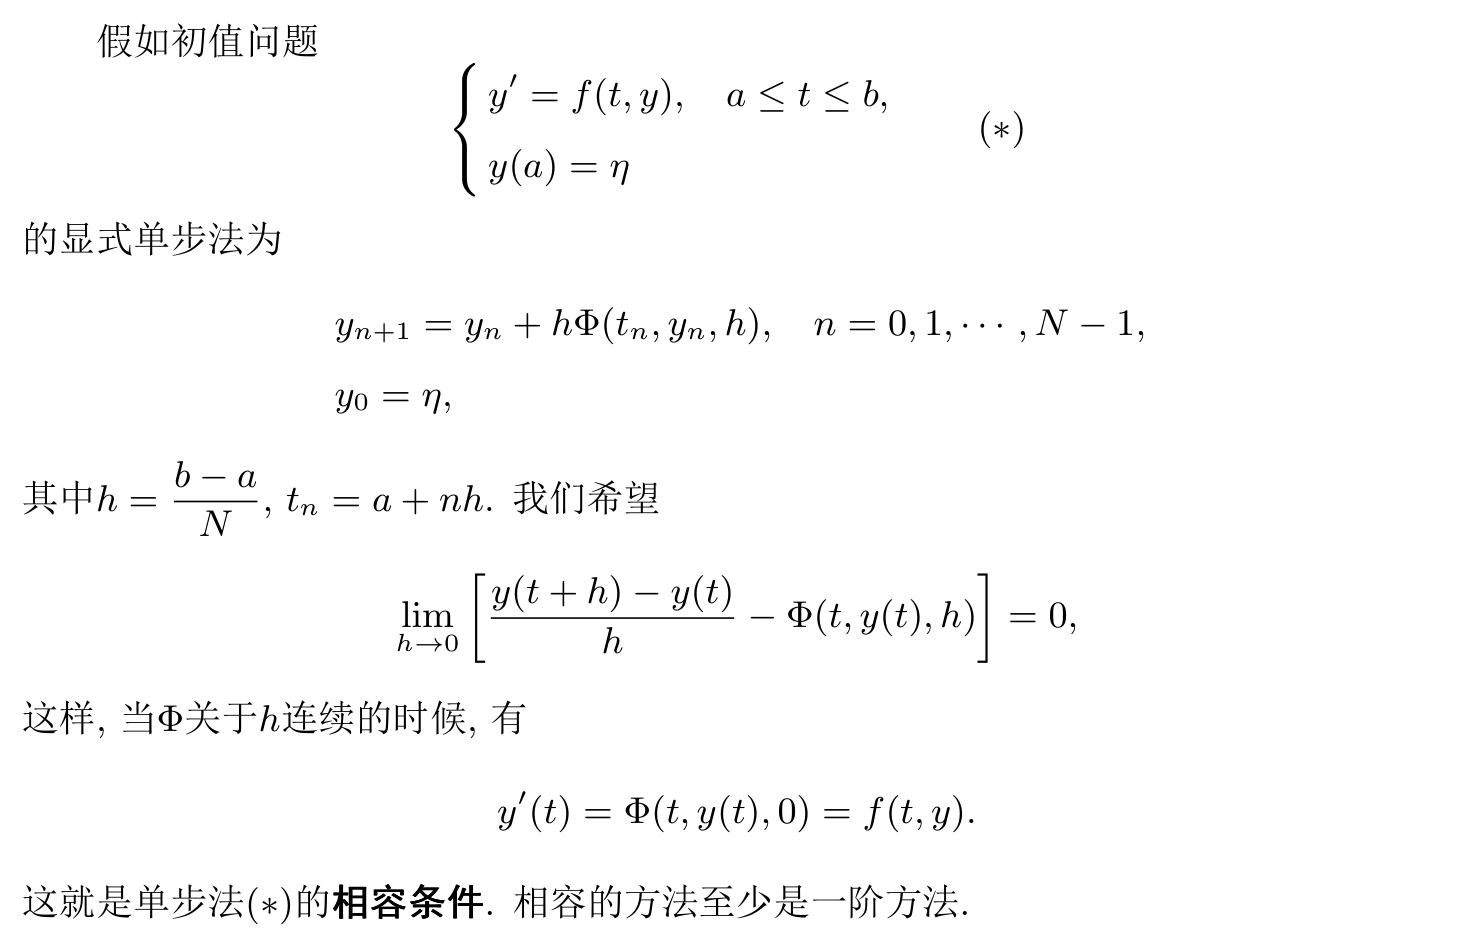
\includegraphics[width=\textwidth]{8-常微分方程数值解-2025051512.png}
% \caption{}
\label{}
\end{figure}
\begin{figure}[H]
\centering
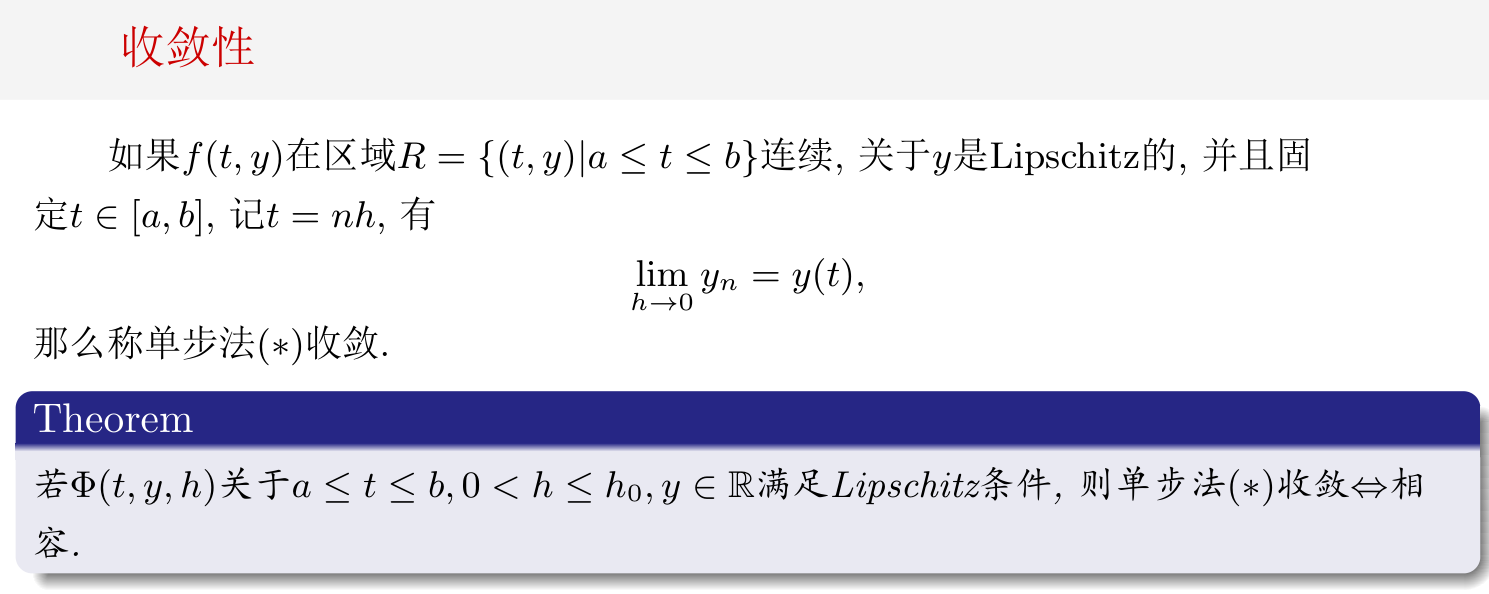
\includegraphics[width=\textwidth]{10-常微分方程数值解-2025051512.png}
% \caption{}
\label{}
\end{figure}

\begin{figure}[H]
\centering
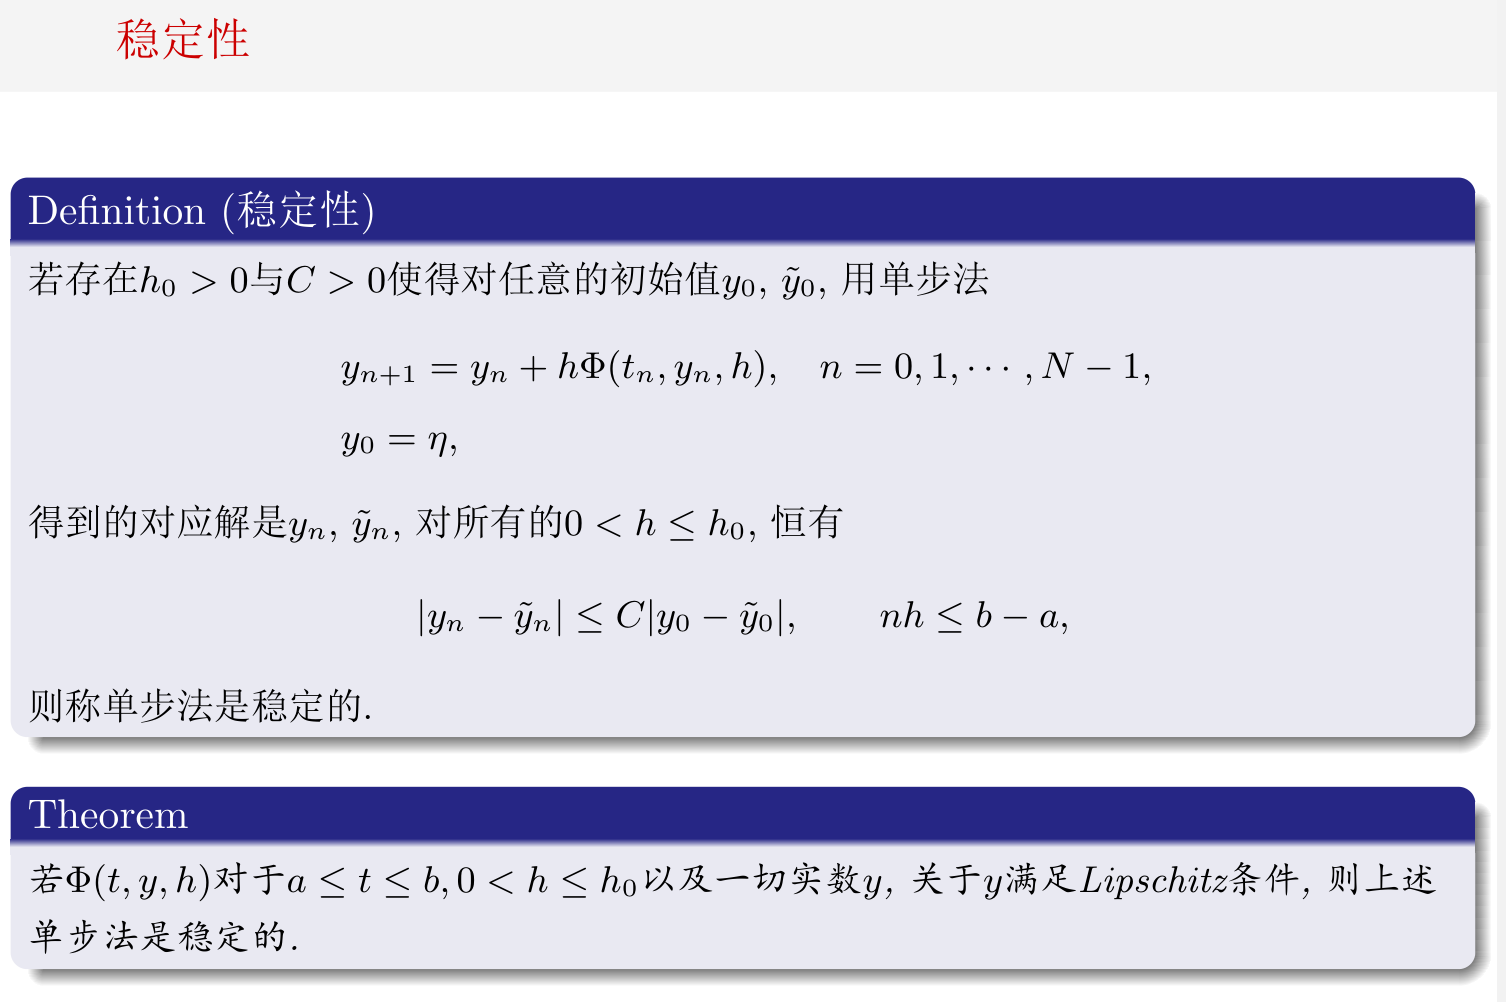
\includegraphics[width=\textwidth]{11-常微分方程数值解-2025051512.png}
% \caption{}
\label{}
\end{figure}

\begin{figure}[H]
\centering
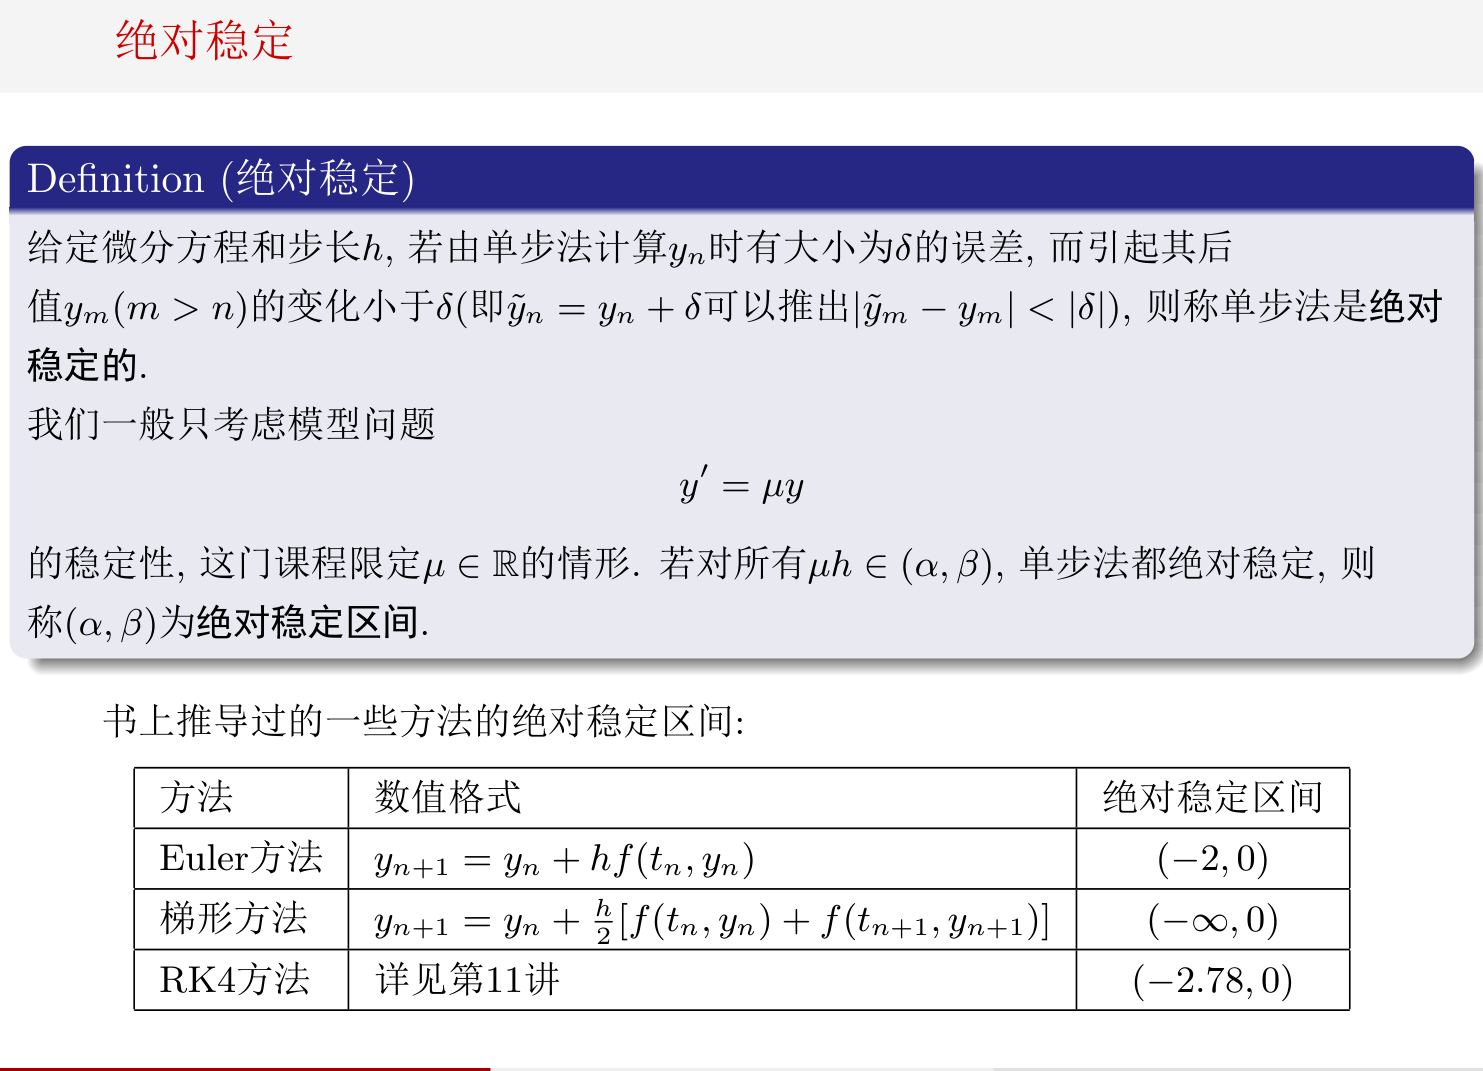
\includegraphics[width=\textwidth]{13-常微分方程数值解-2025051512.png}
% \caption{}
\label{}
\end{figure}

\subsubsection{例题}

\begin{figure}[H]
\centering
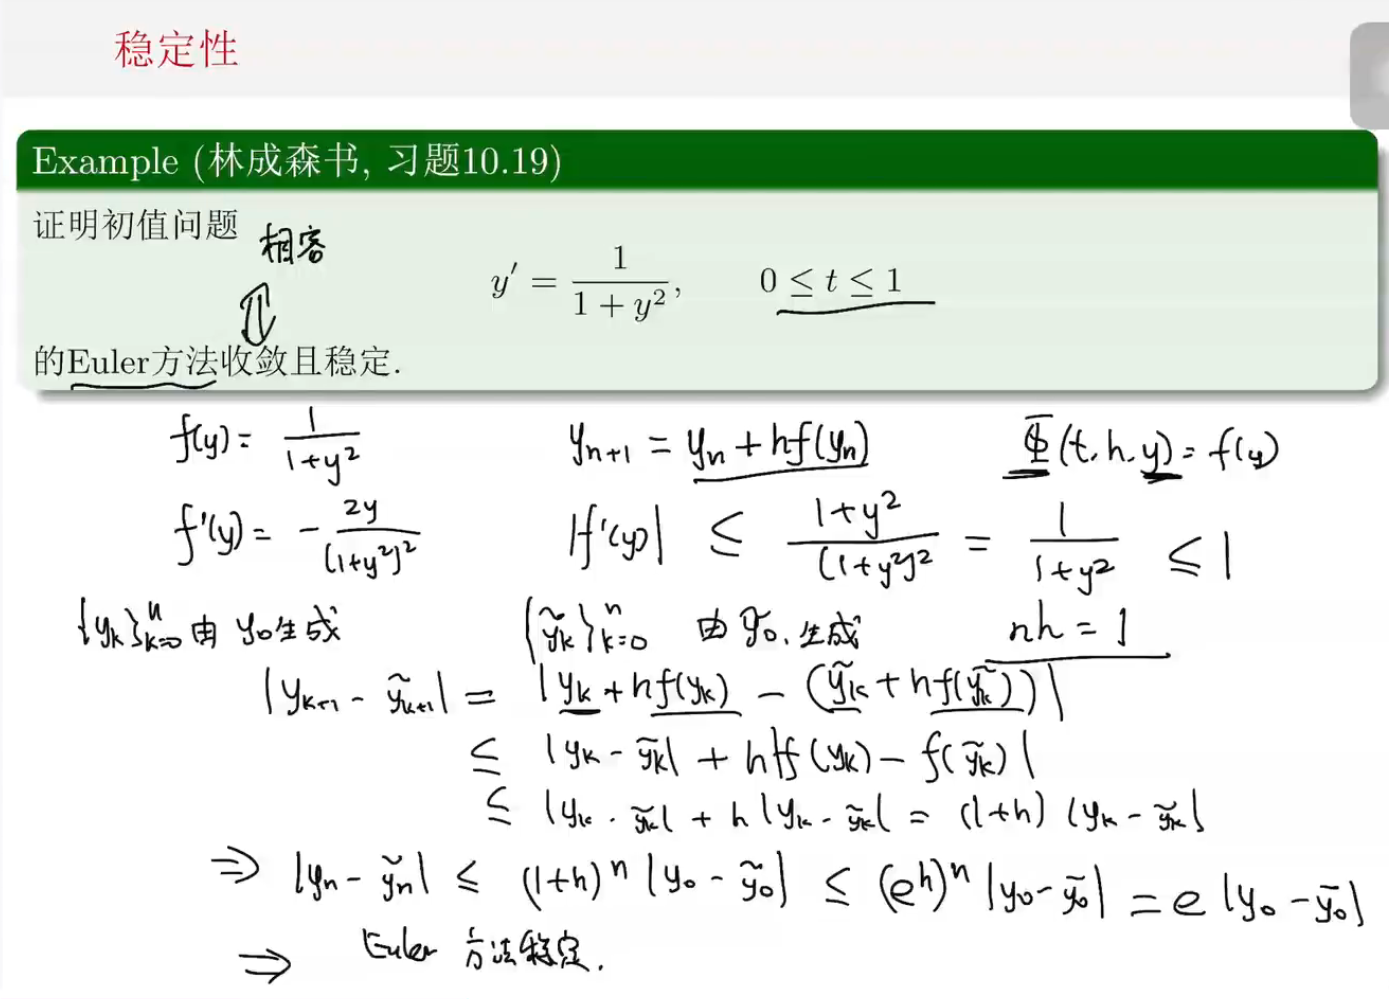
\includegraphics[width=\textwidth]{12-常微分方程数值解-2025051512.png}
% \caption{}
\label{}
\end{figure}
\begin{figure}[H]
\centering
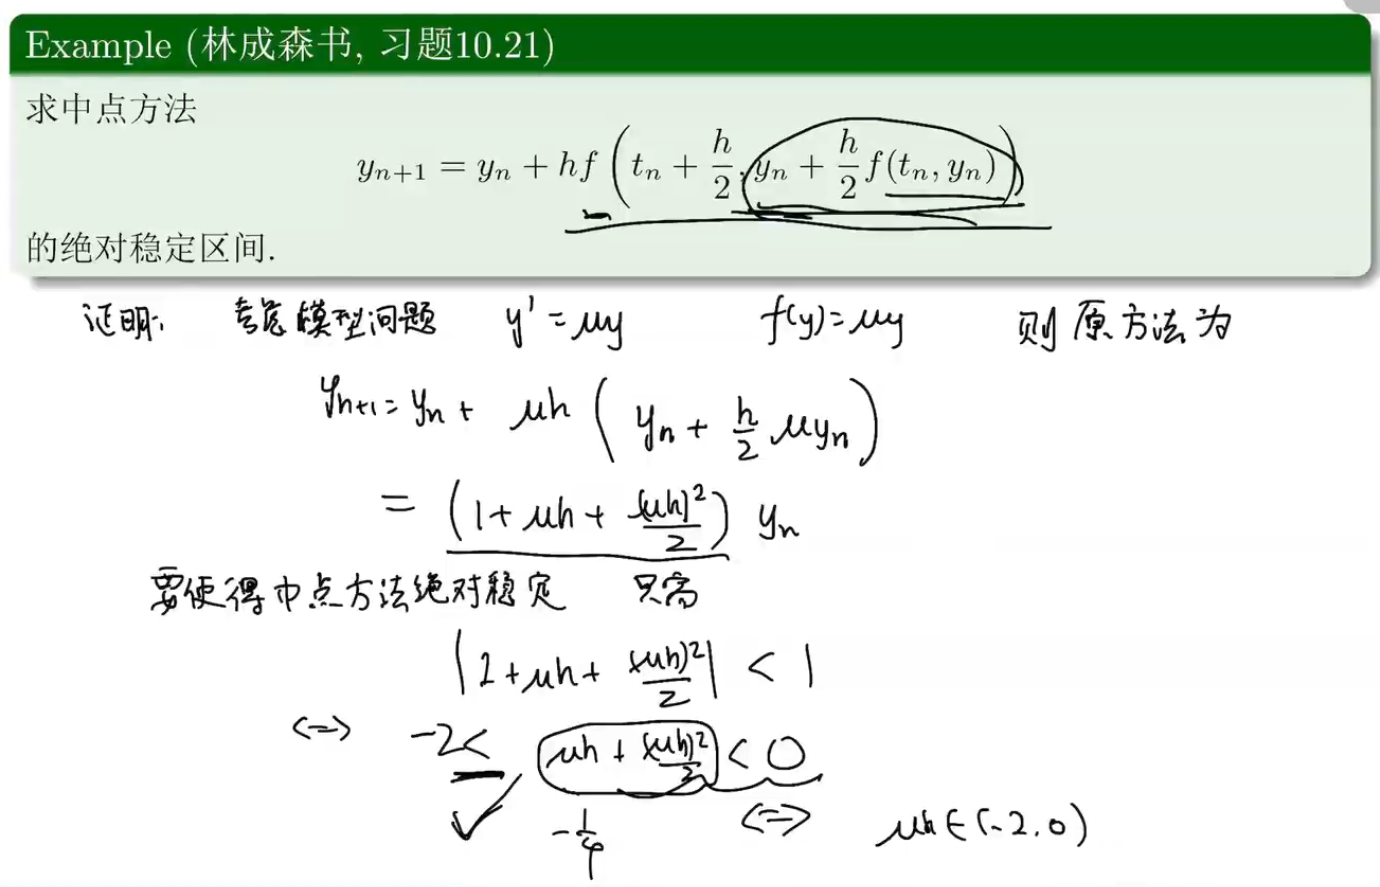
\includegraphics[width=\textwidth]{14-常微分方程数值解-2025051512.png}
% \caption{}
\label{}
\end{figure}

\subsection{多步法}

考虑以下形式的数值方法
\[
y_{n+k}=\sum_{j=0}^{k-1} \alpha_j y_{n+j}+h \sum_{j=0}^k \beta_j f\left(t_{n+j}, y_{n+j}\right), \quad n=0,1, \ldots
\]
其中 $a_j$ 和 $b_j$ 是实常数,$h$ 是步长。这个公式被称为\textbf{线性多步法}。当 $b_k=0$ 时,该方法是\textbf{显式}的;否则,它是\textbf{隐式}的。

改写为
\begin{equation}
\sum_{j=0}^{k} a_j y_{n+j}=h \sum_{j=0}^k b_j f\left(t_{n+j}, y_{n+j}\right), \quad n=0,1, \ldots
\label{7fcebc}
\end{equation}

其中 $a_k\neq0$.

\begin{figure}[H]
\centering
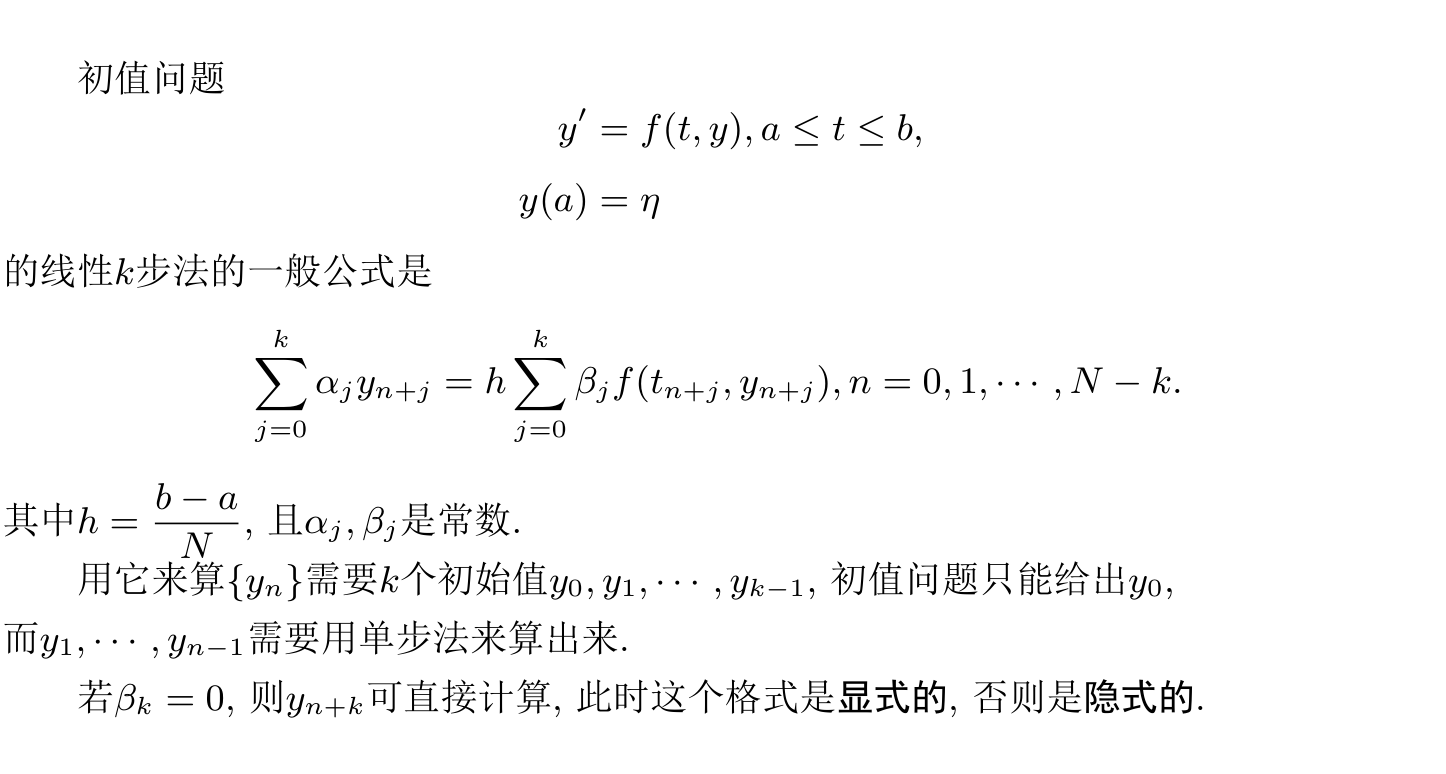
\includegraphics[width=\textwidth]{15-常微分方程数值解-2025051512.png}
% \caption{}
\label{}
\end{figure}
\begin{figure}[H]
\centering
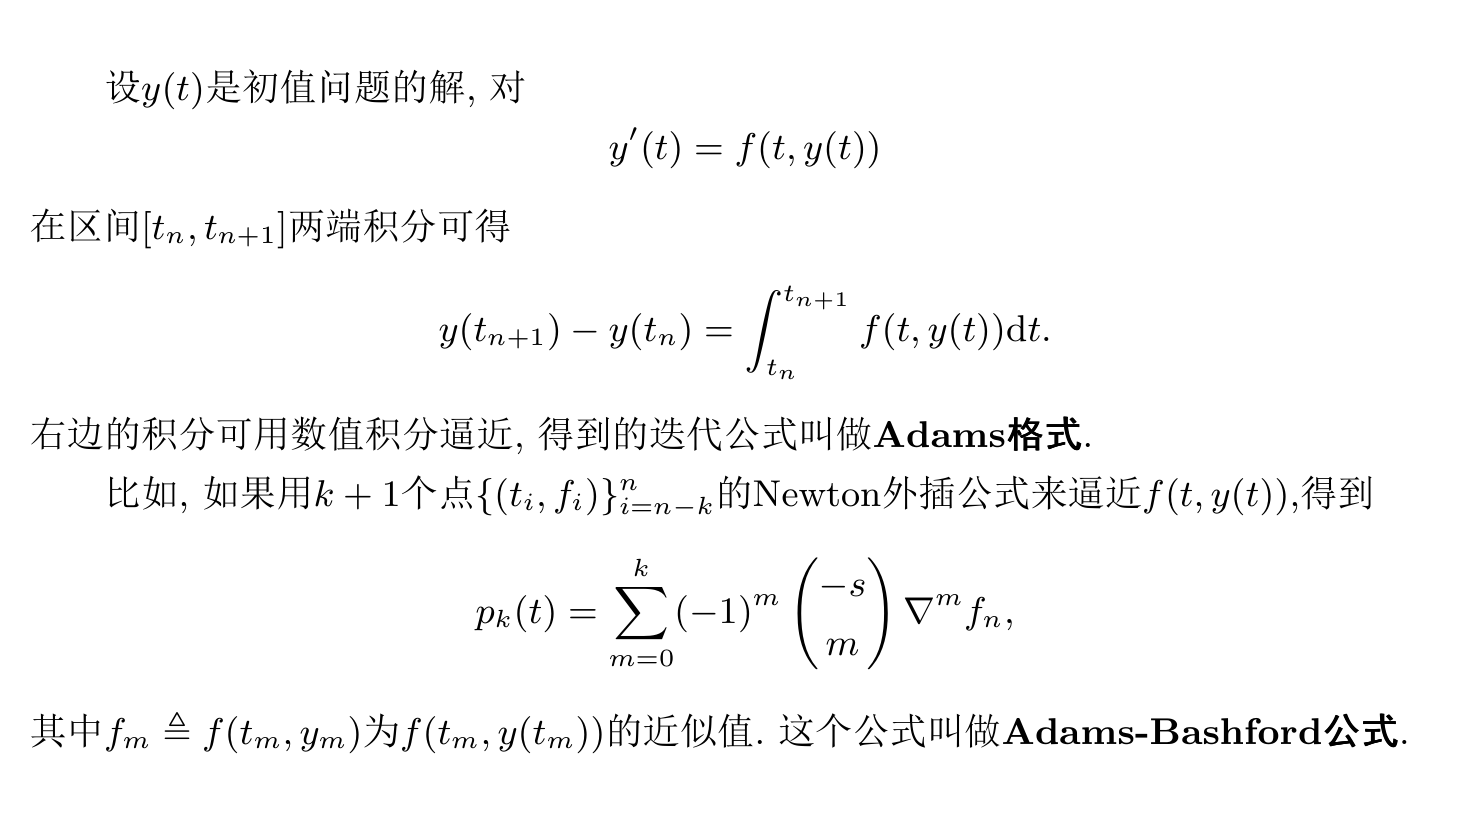
\includegraphics[width=\textwidth]{16-常微分方程数值解-2025051512.png}
% \caption{}
\label{}
\end{figure}

\begin{figure}[H]
\centering
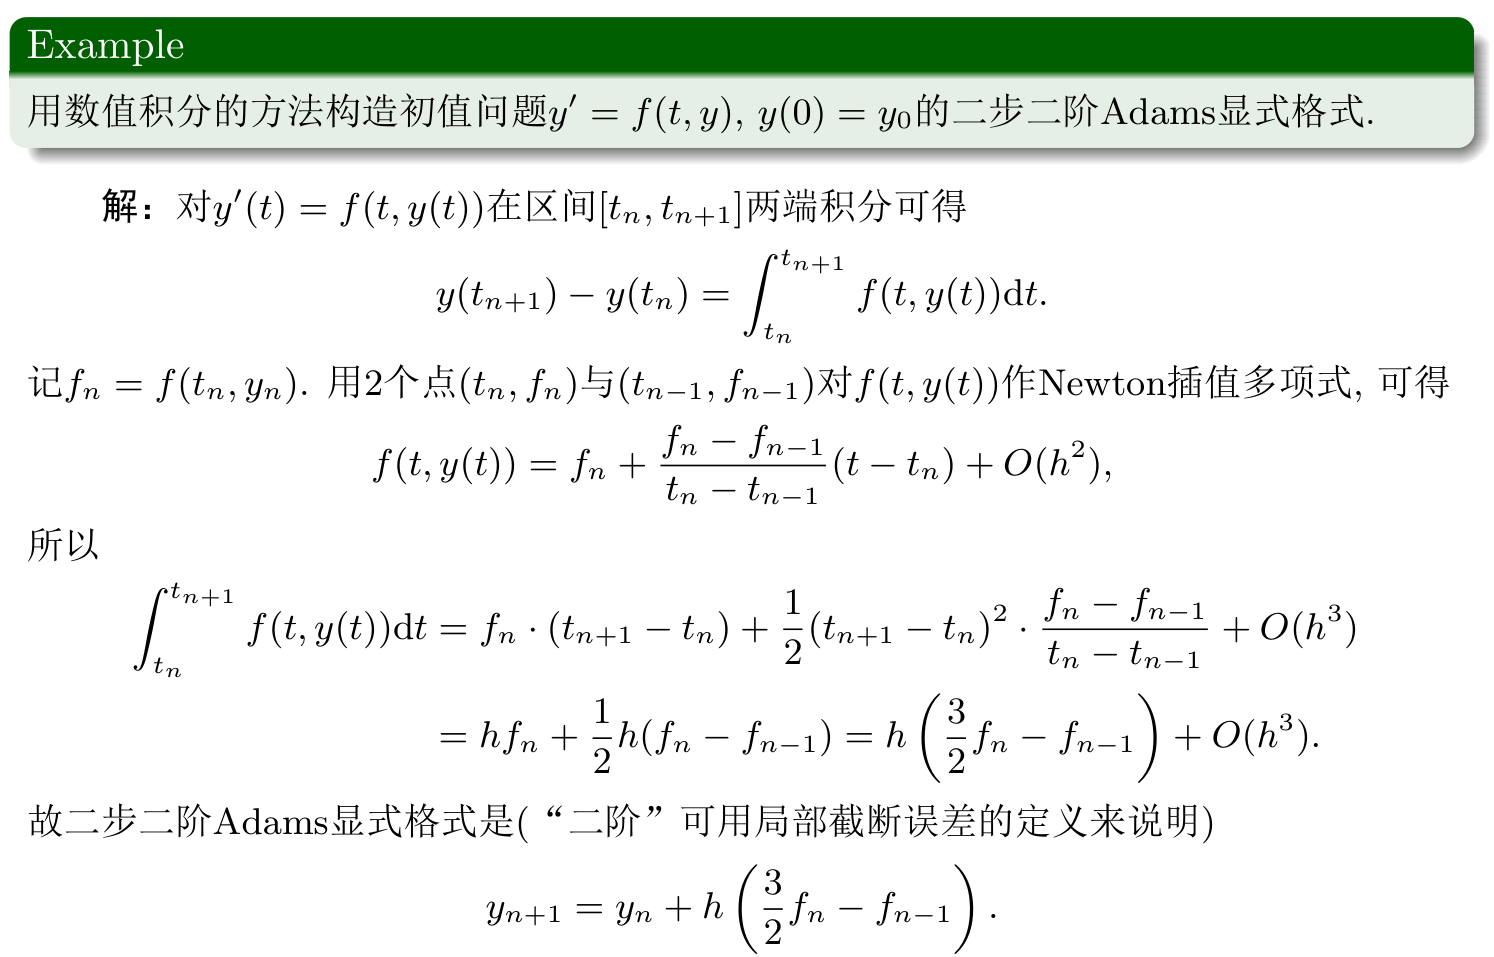
\includegraphics[width=\textwidth]{17-常微分方程数值解-2025051512.png}
% \caption{}
\label{}
\end{figure}
\begin{figure}[H]
\centering
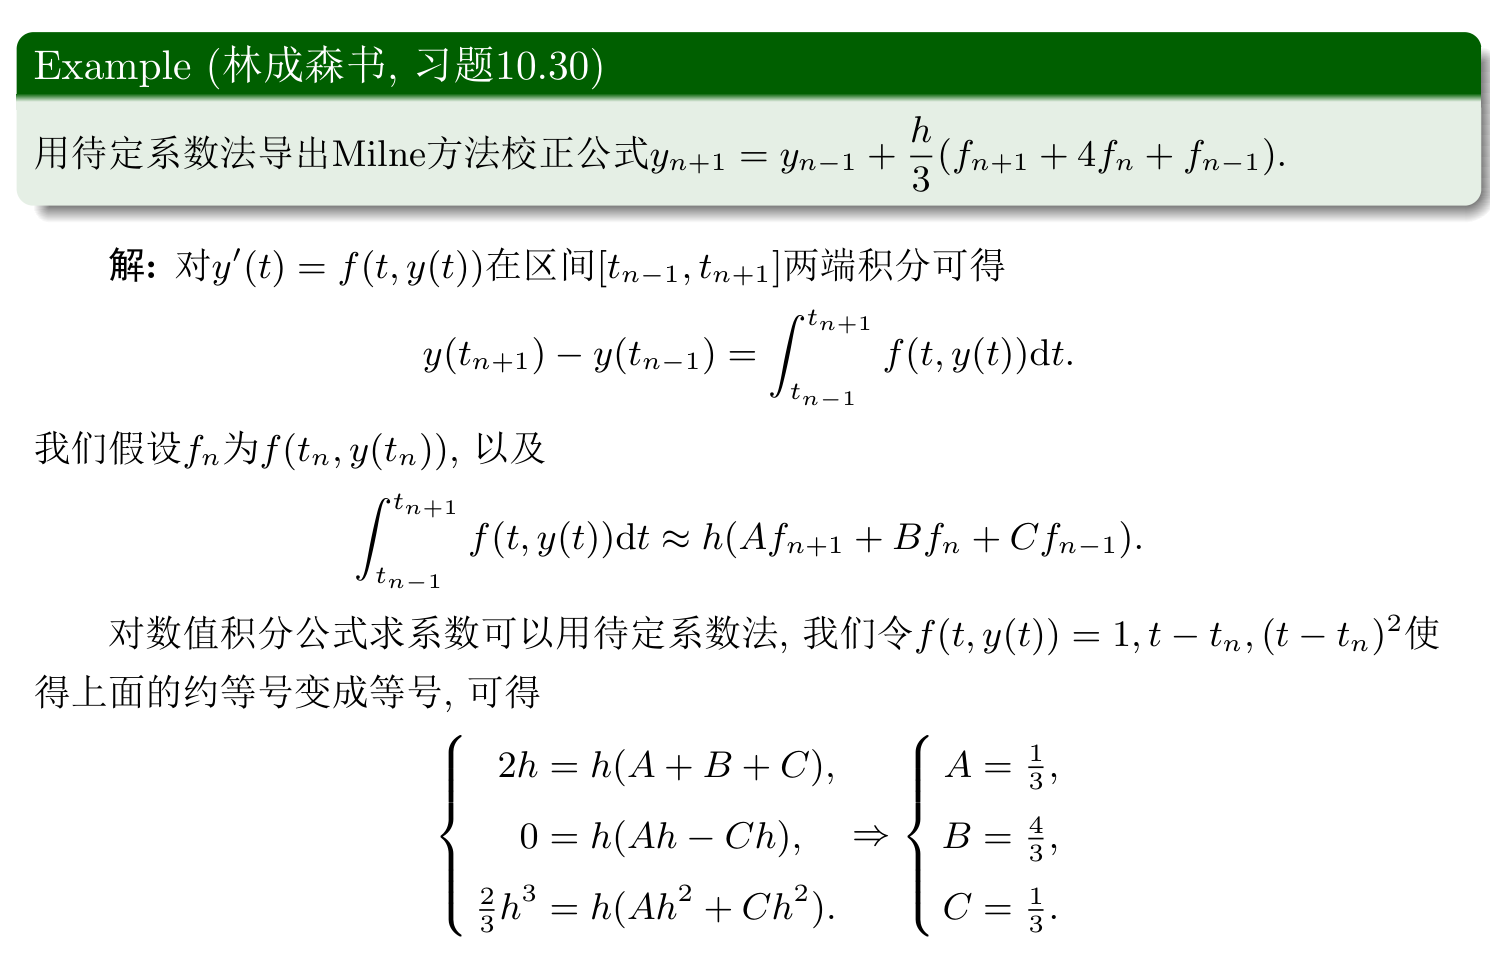
\includegraphics[width=\textwidth]{18-常微分方程数值解-2025051512.png}
% \caption{}
\label{}
\end{figure}

对于线性 $k$ 步法 \cref{7fcebc}, 考虑
\[
\rho(\lambda) = a_k \lambda^k + a_{k-1} \lambda^{k-1} + \cdots + a_1 \lambda + a_0,
\]
\[
\sigma(\lambda) = b_k \lambda^k + b_{k-1} \lambda^{k-1} + \cdots + b_1 \lambda + b_0,
\]
\begin{theorem}[相容条件]
线性 $k$ 步法相容的充要条件是
\[
\rho(1) = 0, \rho'(1) = \sigma(1).
\]
\end{theorem}
\begin{figure}[H]
\centering
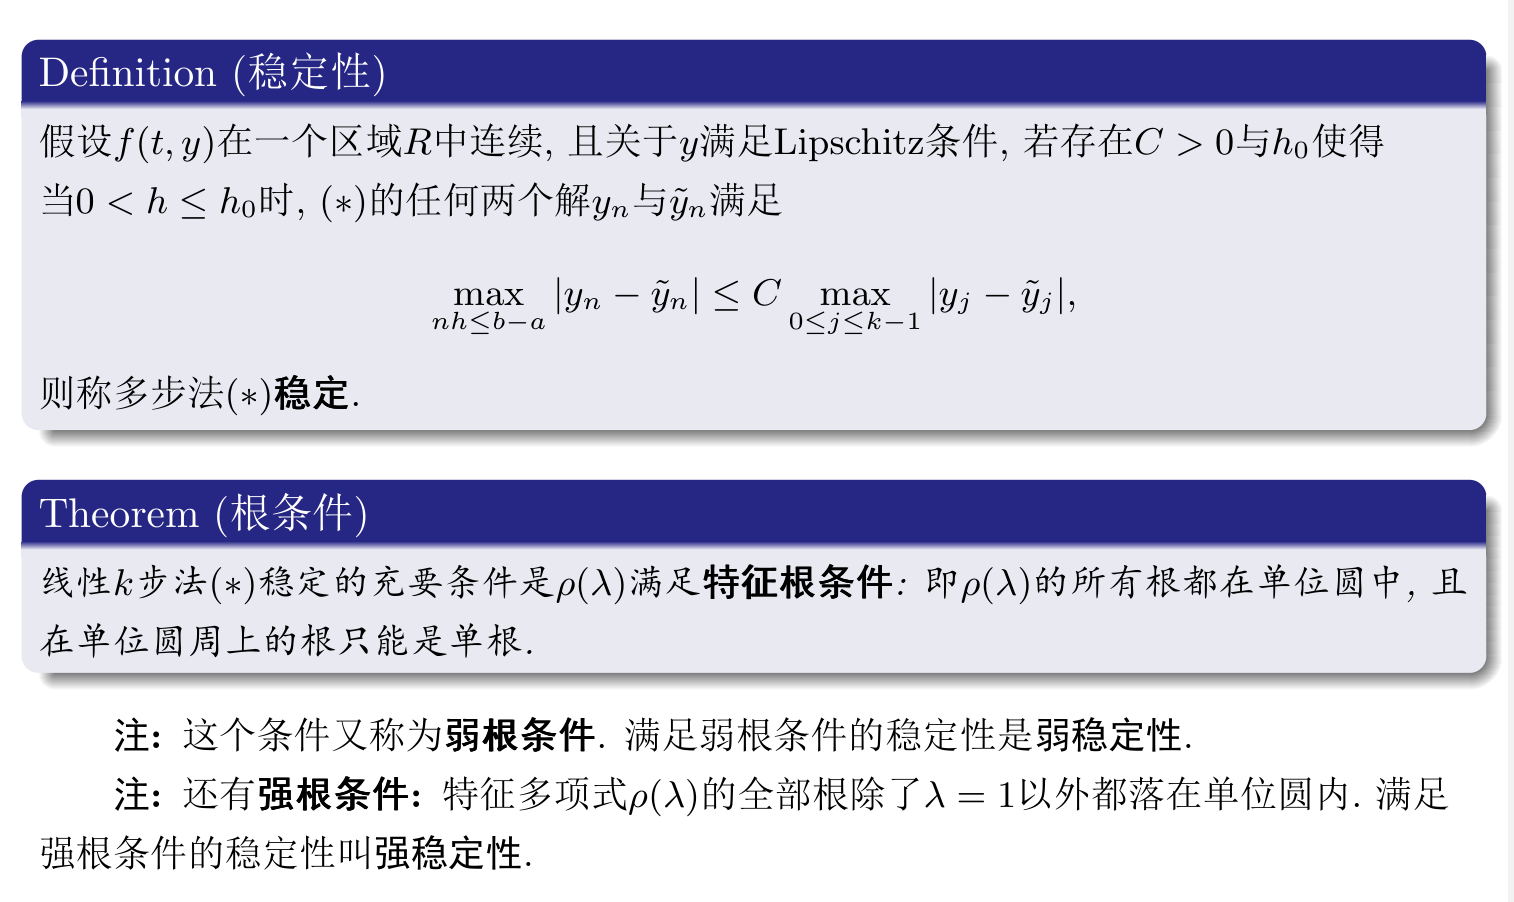
\includegraphics[width=\textwidth]{19-常微分方程数值解-2025051512.png}
% \caption{}
\label{}
\end{figure}
\begin{figure}[H]
\centering
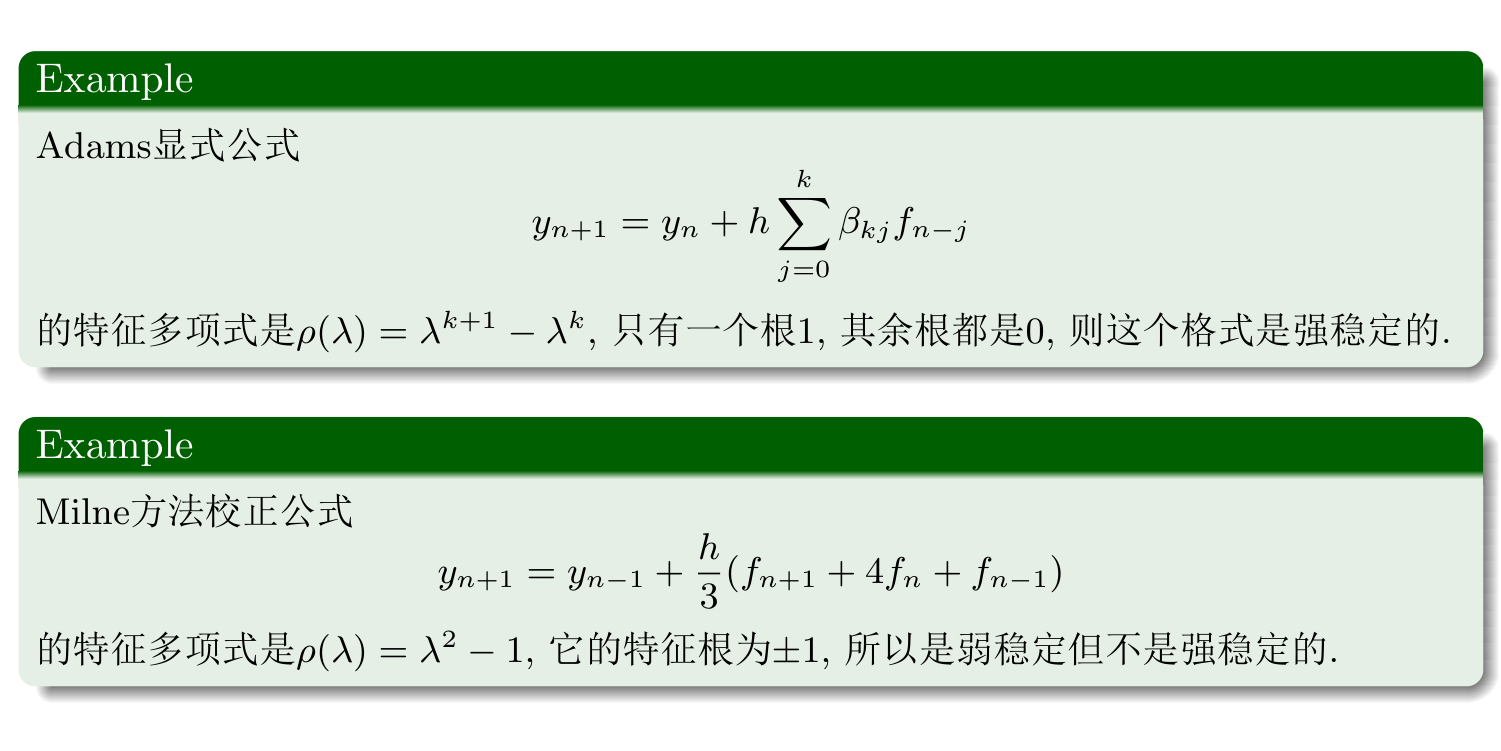
\includegraphics[width=\textwidth]{20-常微分方程数值解-2025051512.png}
% \caption{}
\label{}
\end{figure}

\begin{figure}[H]
\centering
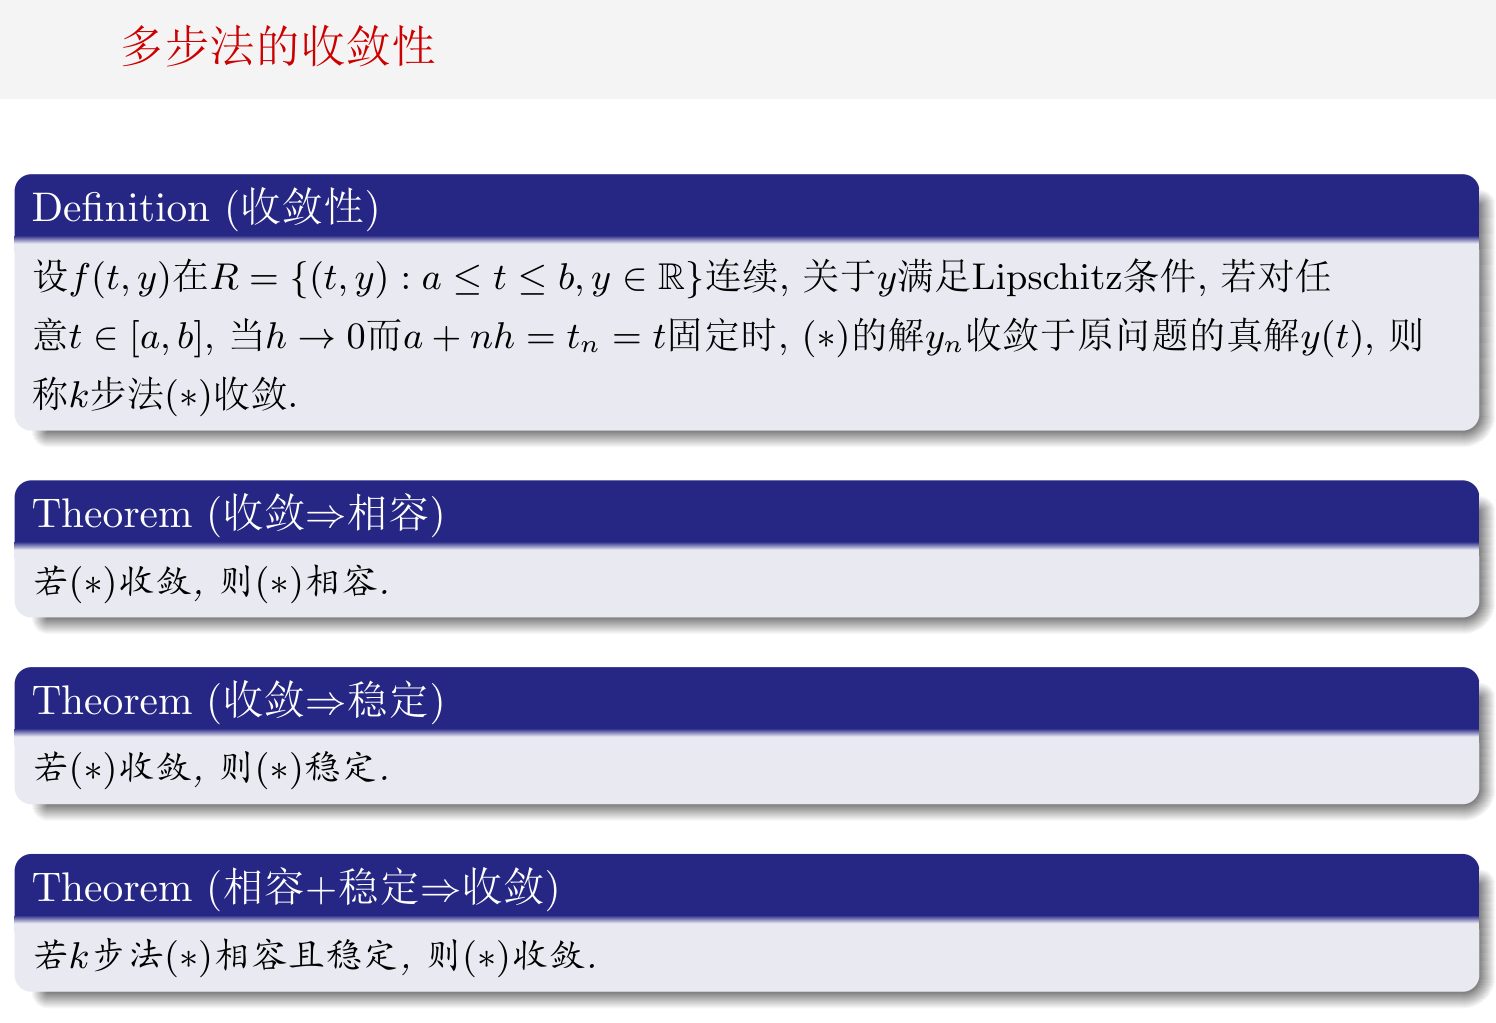
\includegraphics[width=\textwidth]{21-常微分方程数值解-2025051512.png}
% \caption{}
\label{}
\end{figure}
\begin{figure}[H]
\centering
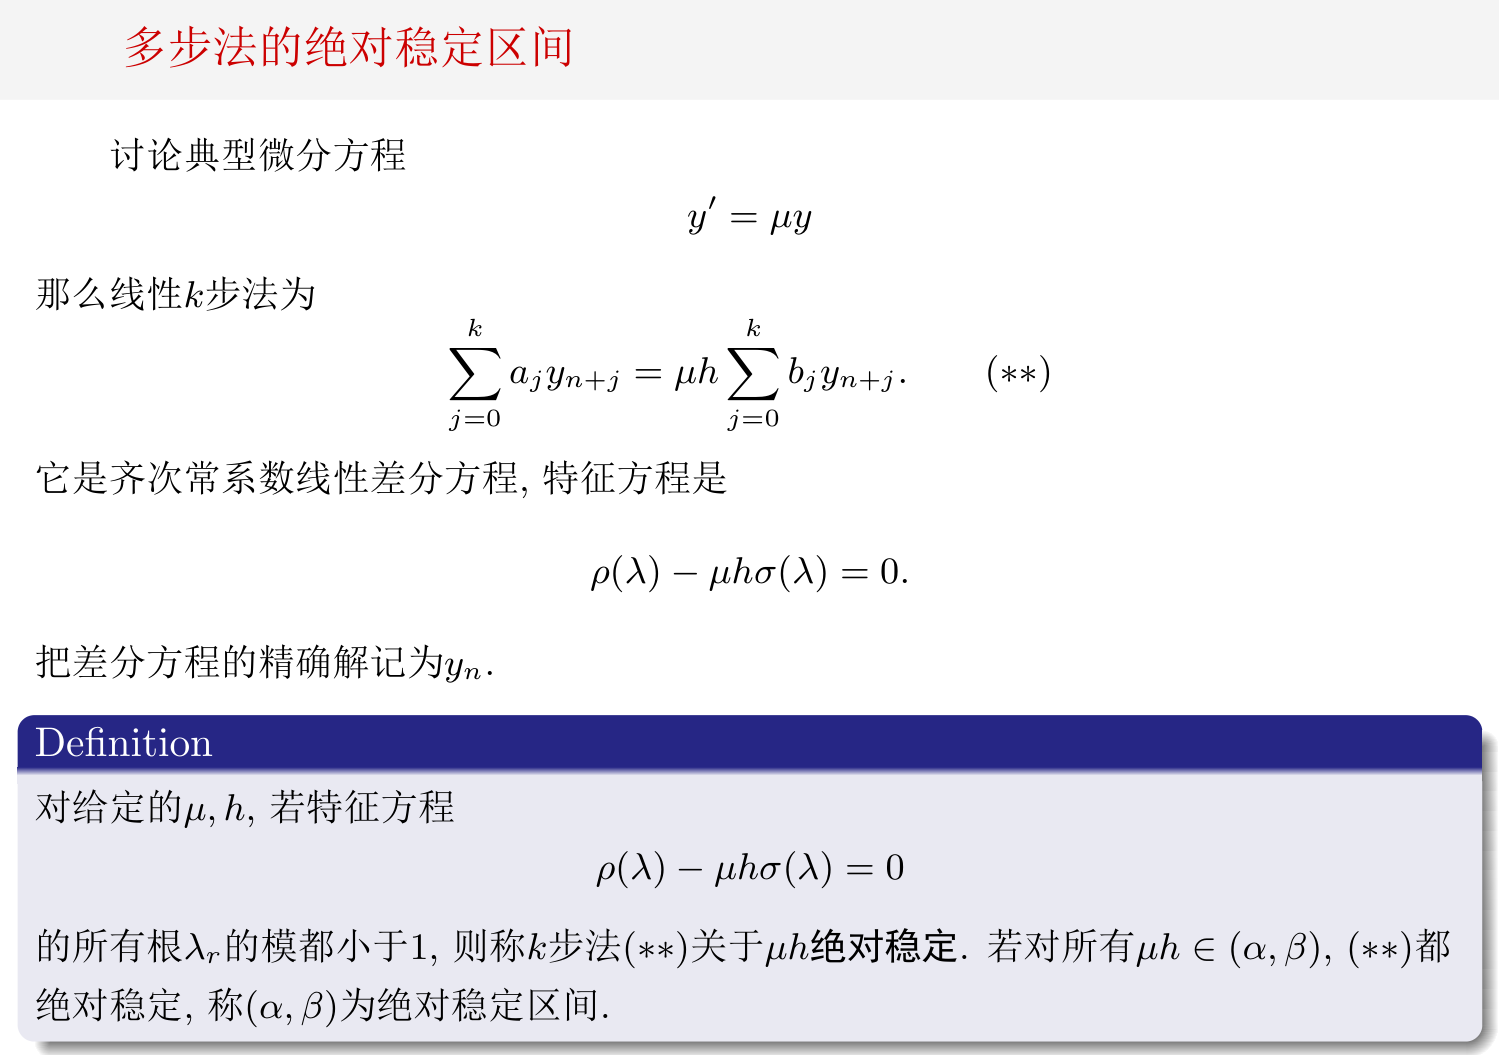
\includegraphics[width=\textwidth]{22-常微分方程数值解-2025051512.png}
% \caption{}
\label{}
\end{figure}

\subsubsection{例题}

\begin{example}
判断求解常微分方程初值问题$y^\prime=f(t,y),y(t_0)=y_0$的线性多步法
\[
y_{n+1}-y_{n-1}=\frac h3(3f_{n+1}-f_n+4f_{n-1})
\]是否收敛,并说明理由.
\end{example}
首先判断零稳定性.
该方法的特征多项式为$\rho(z)=z^2-1$, 其根为$z_1=1, z_2=-1$, 均在单位圆上, 且绝对值为1的根是单根, 故该方法是零稳定的.

接下来判断相容性.
$\rho(1)=0$, $\sigma(1)=\frac{1}{3}(3-1+4)=2$, 故$\frac{\sigma(1)}{\rho'(1)}=\frac{2}{2}=1$.
所以该方法收敛.
